\documentclass{report}

\usepackage[toc]{glossaries}
\usepackage[backend=bibtex]{biblatex}
\usepackage{graphicx}
\usepackage{minted}
\usepackage{lmodern}
\usepackage{tcolorbox}
\usepackage{tabularx}

\newcommand{\code}[1]{\textsf{\ttfamily #1}}
\addbibresource{Rtutorial.bib}
\makenoidxglossaries

\newglossaryentry{dv}{name={discrete variable}, description={A variable that refers to categorical data (ex. color of eyes), as opposed to continuous data (ex. height in mm)}}
\newglossaryentry{cv}{name={continuous variable}, description={A variable that refers to continuous data, i.e. that can take on an infinite number of values (ex. height in mm), as opposed to categorical data (ex. color of eyes)}}
\newglossaryentry{ov}{name={ordinal variable}, description={A variable that refers to categorical data, but where the categories can be ordered (ex. small, medium, large)}}

\author{Myriam Luce}
\title{R: learn by the exercise}

\begin{document}
\maketitle
\tableofcontents

\chapter{Descriptive statistics}
	\section{Tables and figures}
	\subsection{Frequency table (1D) or contingency table (2D)}
If you feel the need to make a table with your data, use a spreadsheet software (Microsoft Excel, LibreOffice Calc, Google Sheets).  ;) R is superior in statistics and (arguably) in figures, but spreadsheets definitely have their uses when it comes to tables.
	\subsection{Pie chart}
A pie chart is a graph that can be used to visually represent proportions of a \emph{\gls{dv}}\footnote{Words in italics are defined in the glossary.}. Note that they have their critics, who recommend never using them for more than two slices, as our brain is bad at comparing the size of slices~\cite{wiki_pie}.

As an example data set, let's use eye color in Pensylvania caucasians~\cite{rebbeck_p_2002}. An excerpt giving the source data is shown in figure~\ref{fig:eyecolor}. Enter the data in your favorite spreadsheet software and save it as a csv (thankfully for you English speakers, there is no need to fiddle with decimal symbol (is it a dot or a comma?) and whether the data is really comma-separated). You should get the following:
\begin{minted}{R}
	blue,green,brown
	255,170,204
\end{minted}
\begin{figure}[h]
	\centering
	\includegraphics[width=0.8\textwidth]{eyecolor.png}
	\caption{Excerpt from \cite{rebbeck_p_2002}.}
	\label{fig:eyecolor}
\end{figure}

R offers various data import options. The most useful I have found were \code{read.csv}\footnote{Words in monospace font refer to R commands. The cheat sheet at the end of the tutorial lists most of those used in this document.} to import csv data and \code{read.fwf} to import fixed-width data. To demonstrate, figure~\ref{fig:data} shows what csv (delimited) and fixed-width data look like side by side.
\begin{figure}[h]
	\centering
	\includegraphics[width=1.0\textwidth]{data.png}
	\caption{Delimited data (left) and fixed-width data (right).}
	\label{fig:data}
\end{figure}

Go ahead and load your small csv into R with \code{read.csv('C:/......data.csv', header=TRUE)}. To avoid messing with default working folder in R settings, I recommend always using the full absolute file path (i.e. starting with C:). Note that you should use the \emph{forward slash "/"} as a path separator, even on Windows. The second parameter, \code{header=TRUE}, tells R that the first line in your file corresponds to the column headers, not actual data. You can then use the function \code{pie(counts, labels)} to produce a pie chart. However, as shown below, a naive approach might displease.
\begin{minted}{R}
> color = read.csv('C:/.../r-tutorial/eyecolor.csv', header=TRUE)
> color
  blue green brown
1  255   170   204
> pie(color, colnames(color))
Error in pie(color, colnames(color)) : 'x' values must be positive.
\end{minted}

You might be scratching your head and wondering which part of 255, 270 or 204 is not positive, and you'd be justified to do so. Here, one must dive into computer programming concerns to understand what is going on. The "not positive" message hints at a problem with the format of the input data. Let's demonstrate:
\begin{minted}{R}
> values = c(255, 170, 204)
> labels = colnames(color)
> pie(values, labels)	# works! produces figure 1.3
> typeof(color)
[1] "list"
> typeof(values)
[1] "double"
> typeof(as.integer(color))
[1] "integer"
> pie(as.integer(color), colnames(color))	# works too!
\end{minted}
\begin{figure}[h]
	\centering
	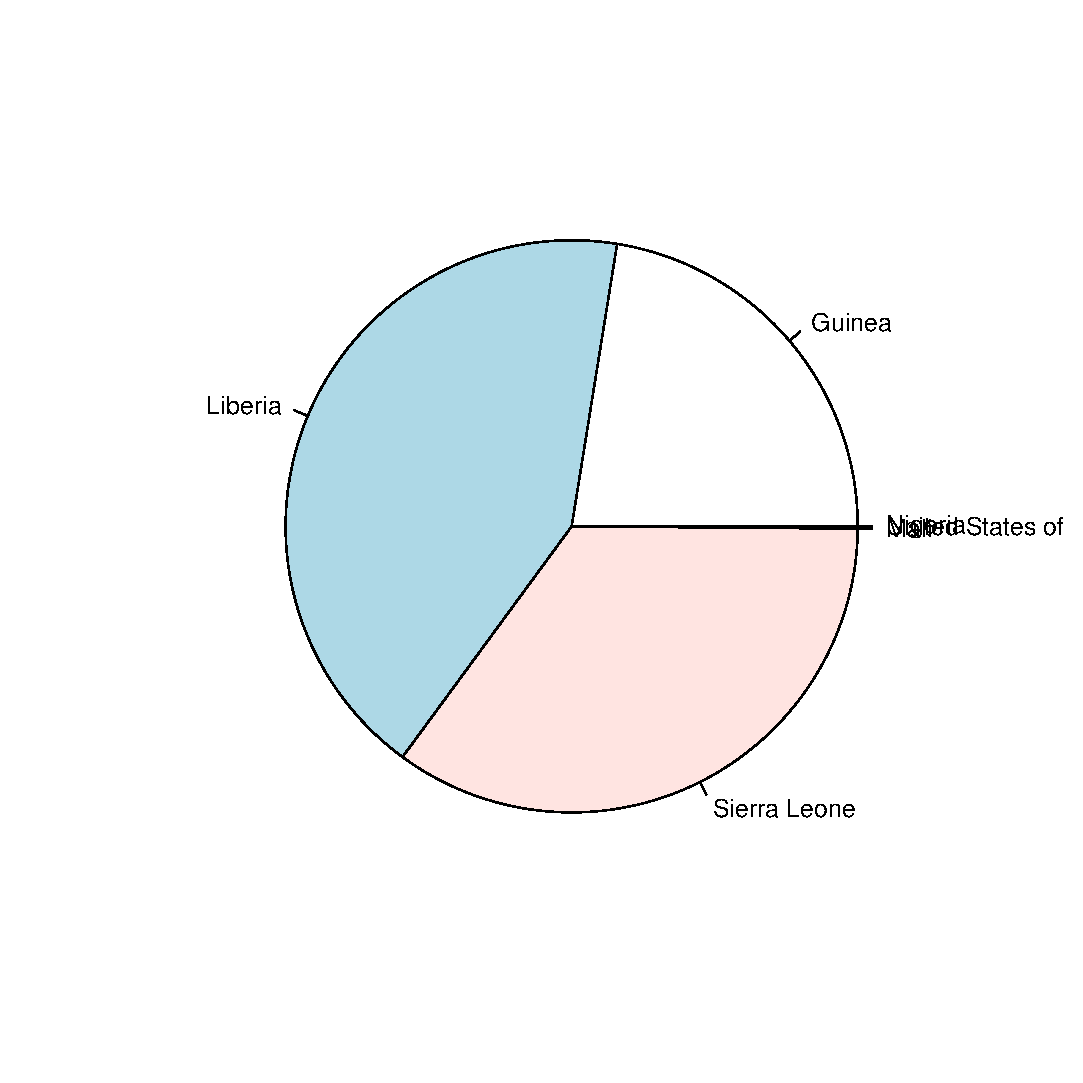
\includegraphics[width=0.8\textwidth]{pie.eps}
	\caption{Eye color among Pennsylvania caucasians.}
\label{fig:pie}
\end{figure}

Technically, \code{read.csv} returns a \code{data.frame}, while \code{pie} only accepts numbers. You can convert your data frame contents to anything reasonable (R will turn "2" into an integer, but not "abc") using the host of \code{as.xyz} functions. Let's take a painful tangent into R types that will hopefully help you later on.

\begin{tcolorbox}[title=R types]
\begin{tabularx}{\textwidth}{>{\bfseries}l X}
Logical: & TRUE or FALSE\\[0.2cm]
Numeric: & real, by the math definition (ex. 12.3). Double is a numeric with better precision.\\[0.2cm]
Integer: & integer, by the math definition (ex. 12).\\[0.2cm]
Character: & text of any length\\[0.2cm]
Factor: & a type that represents a \gls{dv}\\[0.2cm]
Ordered: & a type that represents an \gls{ov}\\[0.2cm]
List: & a 1D collection of "things" (may be strings, numbers, or a mix of them)\\[0.2cm]
Vector: & a 1D collection of things of \emph{one type}\\[0.2cm]
Matrix: & a 2D collection of things of \emph{one type}\\[0.2cm]
Array: & a nD collection of things of \emph{one type}\\[0.2cm]
Data Frame: & a (mostly) 2D collection of things, where each column can be of a different type
\end{tabularx}
For future reference, Quick R gives an excellent introduction on the subject~\cite{quickr}.
\end{tcolorbox}
	\subsection{Bar graph}
	\subsection{Histogram}
	\subsection{Line graph}
	\subsection{Scatter graph}
	\subsection{Box and whiskers graph}
	\section{Numbers}
	\subsection{Center}
	\subsubsection{Mean}
	\subsubsection{Median}
	\subsubsection{Mode}
	\subsection{Dispersion}
	\subsubsection{Range}
	\subsubsection{Variance}
	\subsubsection{Standard deviation}
	\subsubsection{Coefficient of variation}
	\subsubsection{Quartiles and percentiles}
	\subsection{Shape}
	\subsubsection{Skewness}
	\subsubsection{Kurtosis}
	\subsubsection{L-moments}

\chapter{Probabilities}
	\section{Factorial}
	\section{Combinations}
	\section{Permutations}
	\section{Probability Mass/Density Function}

\chapter{Statistics}
	\section{Binomial distribution}
	\section{Multinomial distribution}
	\section{Poisson distribution}
	\section{Inverse binomial distribution}
	\section{Hypergeometric distribution}
	\section{Normal distribution}
	\section{Exponential distribution}
	\section{Gamma distribution}
	\section{c2 distribution}
	\section{Fisher-Snedecor distribution}
	\section{Student’s law}

\chapter{Inferential statistics}
	\section{Student’s test}
	\section{Student’s paired test}
	\section{Bartlett’s test}
	\section{Single-factor ANOVA}
	\section{c2 test}
	\section{Wilcoxon-Mann-Whitney test}
	\section{Kolmogorov-Smirnov test}
	\section{Kruskal-Wallis test}
	\section{Pearson’s test}
	\section{Spearman’s test}
	\section{Kendall’s test}
	\section{Simple linear regression}
	\section{Multiple linear regression}

\chapter{Cheat sheet}

	\section{Plumbing}
\begin{tabbing}
?~~~~~~~~~~~~~ \= ?exact\_function\_name \\
?? \> ??keyword \\
typeof \> typeof(R\_variable) \\
class \> class(R\_variable) \\
str \> str(R\_variable) \\
colnames \> colnames(R\_variable) \\
as.integer \> as.integer(R\_variable)
\end{tabbing}

	\section{Data import and export}
\begin{tabbing}
read.csv~~~~ \= read.csv('delimited\_data.csv', header=TRUE, sep=",", dec=".") \\
read.fwf \> read.fwf('fixed\_width\_data.txt', widths=c(10, 5, 4), header=TRUE, skip=2) \\
write.csv \> write.csv(R\_variable, file='desired\_file\_name.csv', append=FALSE)
\end{tabbing}

\printbibliography

\printnoidxglossaries

\end{document}